% alt: A chain of sixteen dots with four blue sites in the middle braced below as X and three grey sites on each side of them braced below as the buffer T of mD sites; above the chain the two inequalities S(X|T) <= 1/2 S(X) + C (buffered discount) and S(X|T) >= S(X) - 2 S(T) (Araki-Lieb), and below it their consequence S(X) <= 4 S(T) + 2C <= 8 mD log q + 2C.
% Section 5 (Closing the argument), proof of Theorem thm:A and eq:final: the buffered discount eq:discount, S(X|T) <= 1/2 S(X) + C, and the Araki--Lieb lower bound S(X|T) >= S(X) - 2S(T) are combined for the interval X and the buffer T = T_m of at most 2mD sites; the dots are the sites of the chain, the blue dots and brace are the interval X, the two grey braces are the two intervals of the buffer T (mD sites each, drawn for mD = 3), and the unmarked dots are the rest of the chain; no tensor is drawn and no leg is contracted; below, S(X) <= 4S(T) + 2C <= 8mD log q + 2C, with C = 1/2 + C_E/Delta in the note.
\begin{tikzpicture}[x=1cm, y=1cm, line width=0.3pt,
    site/.style={circle, fill=black!55, inner sep=0pt, minimum size=2.6pt},
    xsite/.style={site, fill=blue!65!black},
    brace/.style={decorate, decoration={brace, mirror, amplitude=3pt}},
    lab/.style={font=\small, inner sep=1pt},
    name/.style={font=\scriptsize, text=black!55, inner sep=1pt}]
  % the chain: sites 1..16, X = sites 7..10, T = sites 4..6 and 11..13
  \foreach \i in {1,...,16} {
    \pgfmathsetmacro{\xx}{0.5*(\i-1)}
    \node[site] at (\xx, 0) {};
  }
  \foreach \i in {7,...,10} {
    \pgfmathsetmacro{\xx}{0.5*(\i-1)}
    \node[xsite] at (\xx, 0) {};
  }
  \draw[black!55] (0,0) -- (7.5,0);
  % braces below the chain
  \draw[brace, blue!65!black] (2.77,-0.22) -- (4.73,-0.22)
    node[lab, midway, below=4pt, text=blue!65!black] {\(X\)};
  \draw[brace, black!55] (1.27,-0.22) -- (2.73,-0.22)
    node[lab, midway, below=4pt] {\(T\)}
    node[name, midway, below=14pt] {\(mD\) sites};
  \draw[brace, black!55] (4.77,-0.22) -- (6.23,-0.22)
    node[lab, midway, below=4pt] {\(T\)}
    node[name, midway, below=14pt] {\(mD\) sites};
  % the two inequalities above the chain
  \node[lab, anchor=east] at (3.95, 1.1) {\(S(X\,|\,T)\ \le\ \tfrac12\,S(X)+C\)};
  \node[name, anchor=west] at (4.1, 1.1) {buffered discount};
  \node[lab, anchor=east] at (3.95, 0.65) {\(S(X\,|\,T)\ \ge\ S(X)-2\,S(T)\)};
  \node[name, anchor=west] at (4.1, 0.65) {Araki--Lieb};
  % the consequence below
  \node[lab, anchor=north] at (3.75, -1.05) {\(S(X)\ \le\ 4\,S(T)+2C\ \le\ 8\,mD\log q+2C\)};
\end{tikzpicture}
